% Entity-relationship diagram of the PostgreSQL schema (Section 3.2).
\documentclass[tikz,border=1pt]{standalone}
% =====================================================================
%  Shared style for every diagram in the proposal.
%  Each figure is a standalone TikZ file that \input's this preamble, so
%  all diagrams use the same font family (Computer Modern, T1 -- identical
%  to the LLNCS body text), the same sizes and the same palette.
%
%  Font rule (do not change per figure):
%    node text   \footnotesize  (8 pt)
%    edge labels \scriptsize    (7 pt)
%    titles      \footnotesize\bfseries
%  Figures are drawn at their final width (<= 12.2 cm, the LLNCS text
%  width) and included WITHOUT scaling, so the printed size is the same
%  in every figure.
% =====================================================================
\usepackage[T1]{fontenc}
\usepackage{amsmath,amssymb}
\usepackage{xcolor}
\usepackage{tikz}
\usetikzlibrary{positioning,arrows.meta,shapes.geometric,shapes.multipart,
  fit,backgrounds,calc,shadows,patterns}

% ---- palette ---------------------------------------------------------
\definecolor{cBlue}{HTML}{0B4F8A}    % application / API
\definecolor{cOrange}{HTML}{B4540A}  % processing / services
\definecolor{cPurple}{HTML}{5B3CC4}  % data stores
\definecolor{cGreen}{HTML}{1B7A3A}   % success / output
\definecolor{cRed}{HTML}{B42318}     % error / risk
\definecolor{cGray}{HTML}{5F6672}    % external / neutral
\definecolor{cInk}{HTML}{1F2933}     % text and arrows

\colorlet{fBlue}{cBlue!9}
\colorlet{fOrange}{cOrange!10}
\colorlet{fPurple}{cPurple!9}
\colorlet{fGreen}{cGreen!10}
\colorlet{fRed}{cRed!9}
\colorlet{fGray}{cGray!8}

% ---- fonts -----------------------------------------------------------
\newcommand{\figfont}{\footnotesize}
\newcommand{\lblfont}{\scriptsize}
\newcommand{\code}[1]{\texttt{#1}}

\tikzset{
  every picture/.style={font=\figfont, line join=round, >={Stealth[length=4pt,width=3.4pt]}},
  every node/.append style={execute at begin node={\hyphenpenalty=10000\exhyphenpenalty=10000}},
  base/.style={draw, rounded corners=2pt, line width=0.6pt, align=center,
               inner xsep=3pt, inner ysep=2.5pt, text=cInk, font=\figfont},
  app/.style={base, draw=cBlue, fill=fBlue},
  svc/.style={base, draw=cOrange, fill=fOrange},
  data/.style={base, draw=cPurple, fill=fPurple},
  ok/.style={base, draw=cGreen, fill=fGreen},
  bad/.style={base, draw=cRed, fill=fRed},
  ext/.style={base, draw=cGray, fill=fGray},
  plain/.style={base, draw=none, fill=none},
  db/.style={cylinder, shape border rotate=90, aspect=0.22, draw=cPurple,
             fill=fPurple, line width=0.6pt, align=center, text=cInk,
             minimum height=9mm, font=\figfont},
  decision/.style={diamond, aspect=2.2, draw=cOrange, fill=fOrange,
                   line width=0.6pt, align=center, inner sep=1pt, text=cInk, font=\figfont},
  actor/.style={draw=cInk, fill=fGray, line width=0.8pt, rounded corners=0pt,
                align=center, inner sep=3pt, font=\figfont\bfseries},
  layer/.style={draw=cGray!60, fill=cGray!4, rounded corners=3pt, line width=0.5pt},
  layertitle/.style={font=\lblfont\bfseries, text=cGray, anchor=north west, inner sep=2pt},
  arr/.style={->, draw=cInk, line width=0.6pt},
  darr/.style={->, draw=cGray, line width=0.6pt, dashed},
  biarr/.style={<->, draw=cInk, line width=0.6pt},
  lbl/.style={font=\lblfont, text=cInk, inner sep=1.5pt},
  lblbg/.style={font=\lblfont, text=cInk, inner sep=1.5pt, fill=white},
}

% ---- UML sequence-diagram helpers -----------------------------------
%  \lifeline{id}{x}{label}{bottom y}   head box + dashed life line
%  \msg{x1}{x2}{y}{label}              synchronous call (solid)
%  \ret{x1}{x2}{y}{label}              reply (dashed)
%  \selfmsg{x}{y}{label}               call to self, label on the right
%  \fragment{kind}{guard}{x1}{y1}{x2}{y2}  combined fragment (alt/loop/par)
\newcommand{\lifeline}[4]{%
  \node[app, text width=19mm, minimum height=8.5mm, font=\figfont\bfseries] (#1) at (#2,0) {#3};
  \draw[cGray, dashed, line width=0.5pt] (#1.south) -- (#2,#4);}
\newcommand{\msg}[4]{%
  \draw[arr] (#1,#3) -- node[lbl, above] {#4} (#2,#3);}
\newcommand{\ret}[4]{%
  \draw[darr] (#1,#3) -- node[lbl, above] {#4} (#2,#3);}
\newcommand{\selfmsg}[3]{%
  \draw[arr] (#1,#2+0.12) -- ++(0.3,0) -- ++(0,-0.24) -- ++(-0.3,0);
  \node[lbl, anchor=west, align=left] at (#1+0.35,#2) {#3};}
\newcommand{\fragment}[6]{%
  \draw[cGray, line width=0.5pt] (#3,#4) rectangle (#5,#6);
  \node[anchor=north west, draw=cGray, fill=white, font=\lblfont\bfseries,
        inner sep=1.5pt, line width=0.5pt] at (#3,#4) {#1};
  \if\relax\detokenize{#2}\relax\else
  \node[anchor=north west, font=\lblfont, text=cGray, inner sep=1.5pt] at (#3+0.75,#4) {[#2]};\fi}
\newcommand{\activation}[3]{% x, y top, y bottom
  \draw[draw=cBlue, fill=fBlue, line width=0.5pt] (#1-0.07,#2) rectangle (#1+0.07,#3);}

\usepackage{array}
\newcommand{\pk}[1]{\underline{\smash{#1}}}
\newcommand{\ty}[1]{{\lblfont\textcolor{cGray}{#1}}}
\newenvironment{cols}{\renewcommand{\arraystretch}{1.05}\setlength{\tabcolsep}{2pt}%
  \begin{tabular}{@{}l l@{}}}{\end{tabular}}
\tikzset{
  entity/.style={rectangle split, rectangle split parts=2, draw=cPurple, line width=0.6pt,
    rectangle split part fill={cPurple!16,white}, align=left, inner xsep=3pt, inner ysep=2.5pt,
    text=cInk, font=\figfont, anchor=north west},
  comp/.style={draw=cInk, line width=0.6pt},
}
\begin{document}
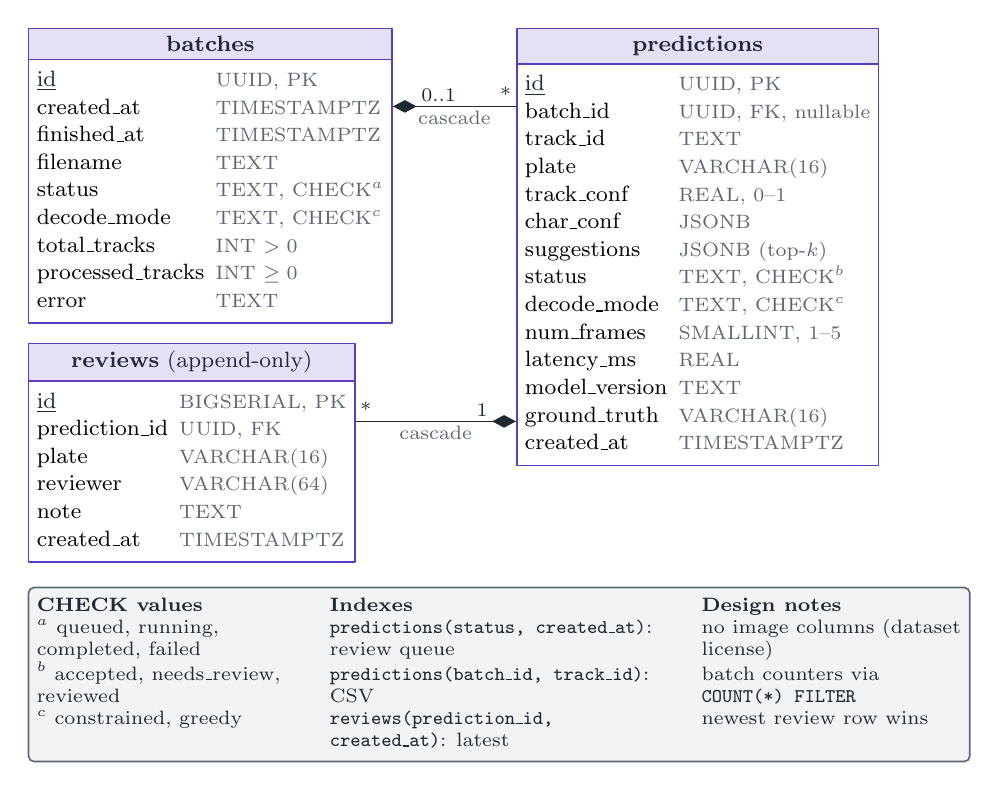
\begin{tikzpicture}
  \node[entity] (bat) at (0,0) {\textbf{batches}\nodepart{two}
    \begin{cols}
      \pk{id}            & \ty{UUID, PK} \\
      created\_at       & \ty{TIMESTAMPTZ} \\
      finished\_at      & \ty{TIMESTAMPTZ} \\
      filename          & \ty{TEXT} \\
      status            & \ty{TEXT, CHECK$^{a}$} \\
      decode\_mode      & \ty{TEXT, CHECK$^{c}$} \\
      total\_tracks     & \ty{INT $>0$} \\
      processed\_tracks & \ty{INT $\ge0$} \\
      error             & \ty{TEXT} \\
    \end{cols}};

  \node[entity] (rev) at (0,-4.0) {\textbf{reviews} (append-only)\nodepart{two}
    \begin{cols}
      \pk{id}            & \ty{BIGSERIAL, PK} \\
      prediction\_id    & \ty{UUID, FK} \\
      plate             & \ty{VARCHAR(16)} \\
      reviewer          & \ty{VARCHAR(64)} \\
      note              & \ty{TEXT} \\
      created\_at       & \ty{TIMESTAMPTZ} \\
    \end{cols}};

  \node[entity] (pre) at (6.2,0) {\textbf{predictions}\nodepart{two}
    \begin{cols}
      \pk{id}            & \ty{UUID, PK} \\
      batch\_id         & \ty{UUID, FK, nullable} \\
      track\_id         & \ty{TEXT} \\
      plate             & \ty{VARCHAR(16)} \\
      track\_conf       & \ty{REAL, 0--1} \\
      char\_conf        & \ty{JSONB} \\
      suggestions       & \ty{JSONB (top-$k$)} \\
      status            & \ty{TEXT, CHECK$^{b}$} \\
      decode\_mode      & \ty{TEXT, CHECK$^{c}$} \\
      num\_frames       & \ty{SMALLINT, 1--5} \\
      latency\_ms       & \ty{REAL} \\
      model\_version    & \ty{TEXT} \\
      ground\_truth     & \ty{VARCHAR(16)} \\
      created\_at       & \ty{TIMESTAMPTZ} \\
    \end{cols}};

  % UML composition: filled diamond on the owner side = ON DELETE CASCADE
  \draw[comp] ([yshift=-10mm]bat.north east) -- ([yshift=-10mm]bat.north east -| pre.west);
  \fill[cInk] ([yshift=-10mm]bat.north east) -- ++(0.15,0.08) -- ++(0.15,-0.08) -- ++(-0.15,-0.08) -- cycle;
  \node[lbl, above right] at ([yshift=-10mm, xshift=3mm]bat.north east) {0..1};
  \node[lbl, above left]  at ([yshift=-10mm]bat.north east -| pre.west) {*};
  \node[lbl, below, text=cGray] at ($([yshift=-10mm]bat.north east)!0.5!([yshift=-10mm]bat.north east -| pre.west)$) {cascade};

  \draw[comp] ([yshift=-10mm]rev.north east) -- ([yshift=-10mm]rev.north east -| pre.west);
  \fill[cInk] ([yshift=-10mm]rev.north east -| pre.west) -- ++(-0.15,0.08) -- ++(-0.15,-0.08) -- ++(0.15,-0.08) -- cycle;
  \node[lbl, above right] at ([yshift=-10mm]rev.north east) {*};
  \node[lbl, above left]  at ([yshift=-10mm, xshift=-3mm]rev.north east -| pre.west) {1};
  \node[lbl, below, text=cGray] at ($([yshift=-10mm]rev.north east)!0.5!([yshift=-10mm]rev.north east -| pre.west)$) {cascade};

  % notes strip
  \node[base, draw=cGray, fill=fGray, font=\lblfont, align=left, anchor=north west, inner sep=3pt]
    at ([yshift=-3mm]rev.south west) {%
    \begin{tabular}{@{}>{\raggedright\arraybackslash}p{33mm}>{\raggedright\arraybackslash}p{43mm}>{\raggedright\arraybackslash}p{33mm}@{}}
    \textbf{CHECK values} & \textbf{Indexes} & \textbf{Design notes}\\
    $^{a}$ queued, running, completed, failed &
    \code{predictions(status, created\_at)}: review queue &
    no image columns (dataset license) \\
    $^{b}$ accepted, needs\_review, reviewed &
    \code{predictions(batch\_id, track\_id)}: CSV &
    batch counters via \code{COUNT(*) FILTER} \\
    $^{c}$ constrained, greedy &
    \code{reviews(prediction\_id, created\_at)}: latest &
    newest review row wins \\
    \end{tabular}};
\end{tikzpicture}
\end{document}
